\documentclass[titlepage]{article}      % Comments after  % are ignored
\usepackage{amsmath,amssymb,amsfonts} % Typical maths resource packages
\usepackage{graphicx}                 % Packages to allow inclusion of graphics
\usepackage{hyperref}                 % For creating hyperlinks in cross references
\usepackage{listings}
\usepackage{float}

\oddsidemargin 0cm
\evensidemargin 0cm
\pagestyle{myheadings}

\markboth{{\small\it Mandelbrot VHDL Viewer}}
{{\small\it Ian Roth} }

\textwidth 15.5cm
\topmargin -1cm
\parindent 0cm
\textheight 24cm
\parskip 1mm

\date{\small\it May 2nd, 2013}
\title{Mandelbrot VHDL Viewer}

\author{ Ian Roth \\
{\small ECE8455 Advanced Digital Design Using FPGAs}}

\begin{document}
\maketitle

\begin{abstract}
The purpose of this project is to demonstrate the use of embedded 9 bit multipliers in a pipeline configuration for the generation of a fractal for VGA output. A Mandelbrot Set is the selected fractal and the output can be zoomed by the user. The completed system makes use of the VGA, SRAM, and push button components of the DE2-115 board.
\end{abstract}

\section{Introduction}
Fractals are mathematical sets bound in a complex plane. The Mandelbrot Set is governed by the equation $z_{n + 1} = z^2_{n} + C$ where $C$ is a constant representing a point in the complex plane. Points in the complex plane in the set are bound, while those outside the set tend toward infinity. The iterations needed to determine that a point is unbounded can be used to colorize an image of the set. The real component, displayed on the x axis, is given by the equation $x_{n+1} = x^2_{n} - y^2 + x{0}$ and the imaginary component in the y axis is $y_{n+1} = 2*x_{n}*y_{n} + y{0}$ where $x{0}$ and $y{0}$ are the $x$ and $y$ components of the constant $C$ respectively. Finally, the real and imaginary components are squared, added together, and compared to the integer value of 4. If the sum of the squares is greater than 4, the point is considered unbounded and the number of iterations is written to memory. Comparing small portions of the Mandelbrot Set with the set as a whole reveals self similar features. This makes "zooming in" an interesting feature of generating the Mandelbrot Set on computer hardware.

FPGAs provide an excellent platform for the computation of fractals due to the possibility of parallelizing much of the mathematical functions. The original plan for the project was to create a parallel structure where calculations for each pixel would be completed on the equivalent of one stage of the pipeline. This was determined to be complex in terms of signaling to both the downstream datapath and to the upstream control logic that completion had occurred. A pipelined architecture is far less complex, but the trade off is that although all multipliers are in the datapath, some may be unused when a point is determined to be out of the set early in the computations.

The project was seen as an opportunity to learn more about fixed point arithmetic in VHDL since it is used in other scenarios such as DSP projects. The project also tests the capabilities of the FPGA and board components to run faster than the 50MHz of the provided clock. Computing the Mandelbrot Set is a well known application of an algorithm in computer science and electrical engineering much like Conway's Game of Life or the Bubble Sort, and knowledge of it may prove useful in settings such as job interviews.
\section{Design}
\subsection{Plan}
As mentioned before the original plan was a parallel architecture. A DRAM interface was also planned, but this was dropped due to issues of timing between sections of the project. The Figure 1 below shows the original plan. The schedule was written with one month for construction of the components and one month for testing.
\begin{figure}[H]
\centering
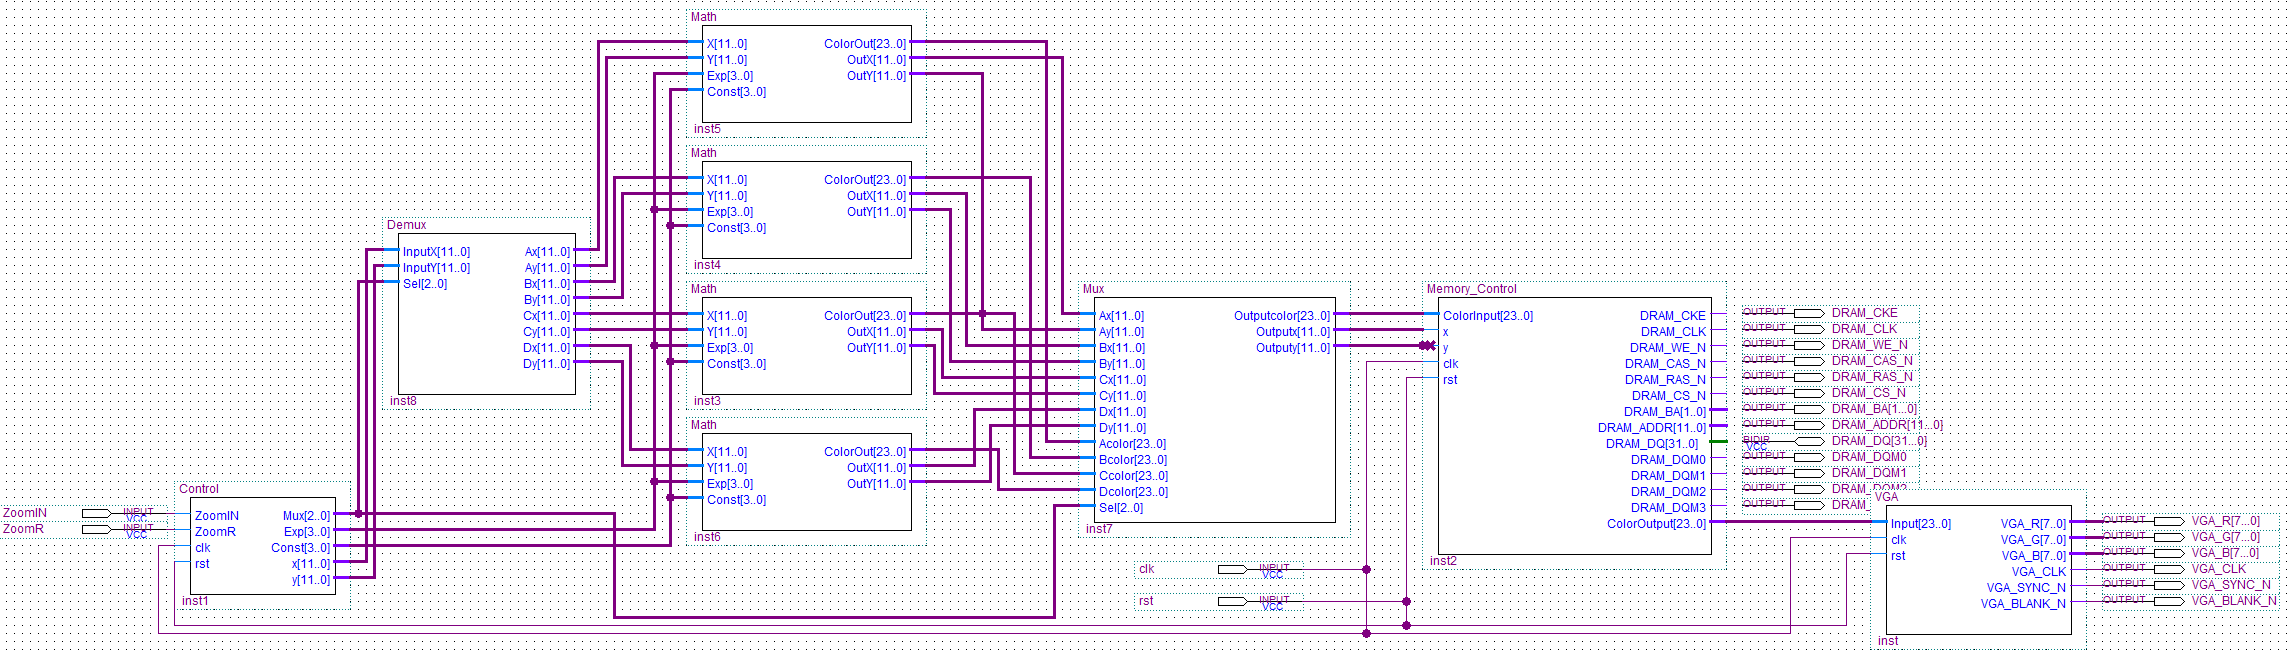
\includegraphics[width=6in]{Diagram}
\caption{Original submitted design.}
\end{figure}
\subsection{Method}
The schedule used built the project from the end of the datapath forward. This was done due to a familiarity with VGA and the ability to continually test on hardware as well as in simulation. For example, the VGA component, despite having nothing to do with the datapath, can be used in a test configuration to determine if acceptable sync and blank signals are outputted to the monitor connected to the DE2-115 board. This is shown in Figure 2 below.
\begin{figure}[H]
\centering
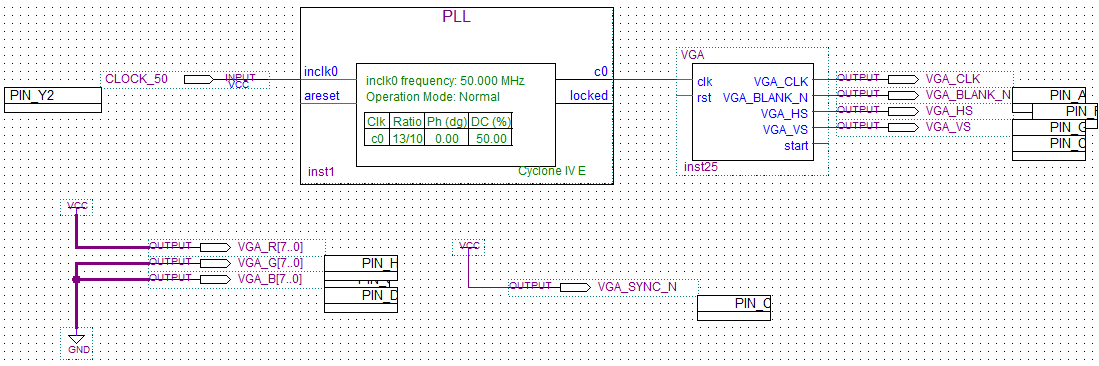
\includegraphics[width=6in]{VGAtest}
\caption{VGA component under test.}
\end{figure}
In the same manner the memory control unit was fed the output of a counter at the iteration input and the system tested for a multicolored gradient output on the monitor. Finally the math and control units were added after simulation and tested with hardware.
\subsection{Realized Design}
\begin{figure}[H]
\centering
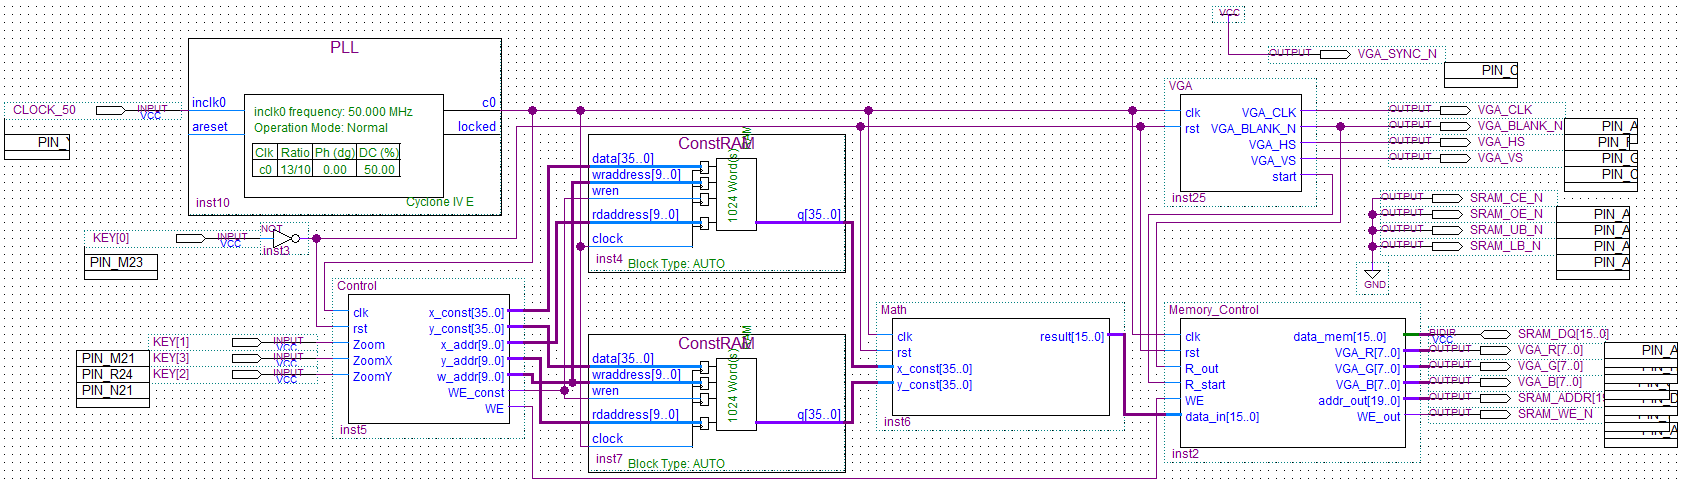
\includegraphics[width=6in]{FinalDiagram}
\caption{Final realized design.}
\end{figure}
\subsubsection{Mandelbrot}
The Mandelbrot component is at the heart of the design and is responsible for all of the computations for one iteration of the Mandelbrot Set calculation. The component is comprised of 3 multiplies, an arithmetic shift (equivalent to logical shift due to left direction), one subtraction and three additions along with an additional addition to keep count of the iterations. X and Y values and constants are all 36 bit fixed point with 1 sign bit, 3 integer bits, and 32 fractional bits. The outputs of the component are clocked, and these registers form the barriers between stages of the pipeline. Below is a listing of the Mandelbrot's architecture.
\begin{lstlisting}
ARCHITECTURE Behavior of Mandelbrot IS
	CONSTANT limit			:sfixed(3 downto 0) := X"2";
	SIGNAL x_sqr, y_sqr	:sfixed(3 downto -32);
BEGIN
	x_sqr <= resize(x_in * x_in, x_sqr);
	y_sqr <= resize(y_in * y_in, y_sqr);
	Process(clk,rst)
	BEGIN
		IF (clk'EVENT and clk = '1') THEN
			IF (rst = '1') THEN
				iteration_out <= X"0000";
				done_out <= '0';
			ELSE
				x_out <= resize(x_sqr - y_sqr + x_const, x_sqr);
				y_out <= resize(((x_in * y_in) sll 1) + y_const, y_sqr);
				x_const_out <= x_const;
				y_const_out <= y_const;
				IF (done_in = '1') THEN
					done_out <= '1';
					iteration_out <= iteration_in;
				ELSE
					IF (resize(x_sqr + y_sqr, x_sqr) > limit) THEN
						done_out <= '1';
						iteration_out <= iteration_in;
					ELSE
						done_out <= '0';
						iteration_out <= iteration_in + 1;
					END IF;
				END IF;
			END IF;
		END IF;
	END PROCESS;
END Behavior;
\end{lstlisting}
\subsubsection{Math}
The math unit contains 23 Mandelbrot pipeline stages in a GENERATE statement and 1 initial stage. Nothing in the math unit is clocked, however the clk and rst signals must be fed to the Mandelbrot units. The GENERATE statement is listed here:
\begin{lstlisting}
gen_math:
FOR i IN 1 TO 23 GENERATE
	stageX: Mandelbrot PORT MAP(x_const => x_const_array(i-1),
		y_const => y_const_array(i-1), x_in => x_array(i-1),
		y_in => y_array(i-1), iteration_in => result_array(i-1),
		done_in => done_array(i-1), clk => clk, rst => rst,
		x_const_out => x_const_array(i),
		y_const_out => y_const_array(i), x_out => x_array(i),
		y_out => y_array(i), iteration_out => result_array(i),
		done_out => done_array(i));
END GENERATE gen_math;
\end{lstlisting}
Note that all but the done array is an array of STD\_LOGIC\_VECTORS or signed fixed values. Inputs to the initial stage are from Math unit inputs and thus are not addressable in the arrays. Outputs from the Math unit are continuous assignments from the 23rd locations in the arrays.
\subsubsection{Memory Controller}
Memory control has been simplified from the original design with the use of the SRAM rather than the SDRAM found on the DE2-115 board. Running the SDRAM would require a clock of 133MHz, which is incompatible with the 65MHz clock necessary for the VGA output. A queue might have been possible, but determining the necessary queue length, use of memory cycles, and simulation would have been difficult. The SRAM controller is very simple. The write enable supersedes read operations. Below is a table of input descriptions.
\begin{table}[H]
\centering
\framebox[5in]{\begin{tabular}{r | l }
$Name$ & $Description$ \\ \hline
clk&Global clock\\
rst&Global reset on high\\
R\_out&Read a pixel out on clock tick, triggered by blank signal from VGA.\\
R\_start&Reset read address to zero, triggered by both sync signals from VGA.\\
WE&Write value to address held in write address.\\
data\_in&Iteration count from math pipeline, it is written when WE is high.\\
\end{tabular}}
\caption{Inputs of the memory controller}
\end{table}
Of note in the VHDL is the way in which the output is handled. The accessed read location in memory is compared to the number of iterations. If they are the same the pixel is displayed as black, and some RGB value based on the iterations otherwise.
\begin{lstlisting}
IF (data_mem = iterations) THEN -- blank pixel if in set
	VGA_R <= X"00";
	VGA_G <= X"00";
	VGA_B <= X"00";
ELSE -- display iterations away from set in form of pixel color
	VGA_R <= do(15) & do(12) & do(9)  & do(6) & do(3) & do(0) & "11";
	VGA_G <= do(13) & do(10) & do(7) & do(4) & do(1) & "111";
	VGA_B <= do(14) & do(11) & do(8) & do(5) & do(2) & "111";
END IF;
\end{lstlisting}
\subsubsection{Control}
The control unit is one half of the control logic, the other detached half being the VGA unit. The control unit is a finite state machine with seven states aligned in a cycle. User input, besides the reset signal, is only considered once the constants and iteration values are written to memory. The states are described as follows.
\begin{table}[H]
\centering
\framebox[5in]{\begin{tabular}{r | c | l }
$State$ & $Period$ & $Description$ \\ \hline
A&1 clk cycle&Output first constants.\\
B&1 clk cycle&First value calculated in pipeline.\\
C&23 clk cycles&Wait for value to propagate through pipeline.\\
D&1000 clk cycles&Start writing values to SRAM.\\
E&785408 clk cycles&Stop writing constants.\\
F&unlimited&Stop writing to SRAM, wait for user input.\\
G&unlimited&Go to stage A when zoom button released.\\
\end{tabular}}
\caption{Control logic finite state machine stage listing}
\end{table}
The zoom functionality is confined to one of four quadrants. This simplifies the math required to calculate the space spanned in the real and imaginary axes. Three pushbuttons are used to determine the location in both axes and to initiate the zoom. The only other user input to the control logic is the synchronous reset function. The outputs are a bit more complex. Along with signals to initiate memory writes and memory addressing, the x and y constants at the start of the datapath are generated by the control logic.
\begin{table}[H]
\centering
\framebox[4in]{\begin{tabular}{r | l }
$Name$ & $Description$ \\ \hline
x\_const&X axis constant for pixel.\\
y\_const&Y axis constant for pixel.\\
x\_addr&Read address for x axis constants.\\
y\_addr&Read address for y axis constants.\\
w\_addr&Write address for both x and y constants.\\
WE\_const&Write enable for constant memory.\\
WE&Write enable for SRAM (iterations).\\
\end{tabular}}
\caption{Control logic output signals}
\end{table}
\subsubsection{VGA}
The VGA unit operates independently of the control logic unit and uses only the global clock and reset as inputs. The outputs directly feed the onboard VGA controller as well as the memory controller. The ANDing of the inverse of the horizontal and vertical sync signals is used to reset the read address in the memory controller. The blank signal indicates to the memory controller that a value should be read from memory and the read address incremented.
\section{Results}
\subsection{Simulation}
Simulation was carried out on critical components of the datapath and the control logic unit using the Modelsim tool. All available Altera Cyclone libraries were loaded for the most realistic simulations possible. The VGA and memory controller worked right away on the hardware with test inputs and thus were never simulated. Fixed point libraries were required for simulation, and conversions of fixed point values to logic vectors were removed due to compiler issues in Modelsim.
\subsubsection{ConstRAM}
The megawizard generated RAM block for holding the constants was tested to ensure that it would work in the design as expected. As shown below reading can be completed one clock cycle after writing, and reads can occur on every clock cycle as required.
\begin{figure}[H]
\centering
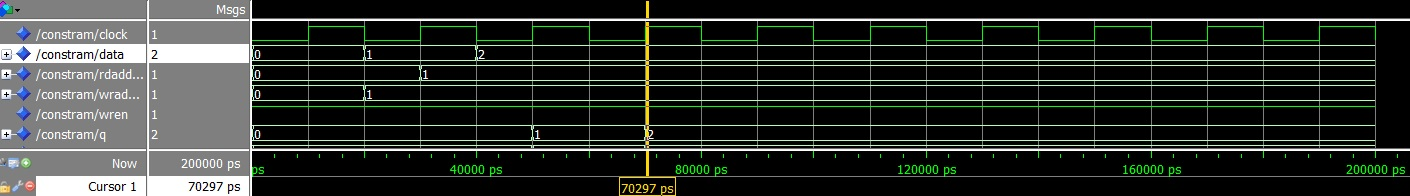
\includegraphics[width=6in]{ConstRAM}
\caption{RAM for constants under test.}
\end{figure}
\subsubsection{Control}
The control unit was repeatedly simulated until the proper sequence of output was generated. In some cases the simulation differed from the expected results. For example it was expected that the transition from state D to E should occur when the constant write counter was at 1023, but it was found that the value should actually be 1022. Zoom input was not tested in the control unit due to the time required to simulate the writing of all 786432 pixels before user input is considered. This lead to some debugging of the control logic using the hardware.
\begin{figure}[H]
\centering
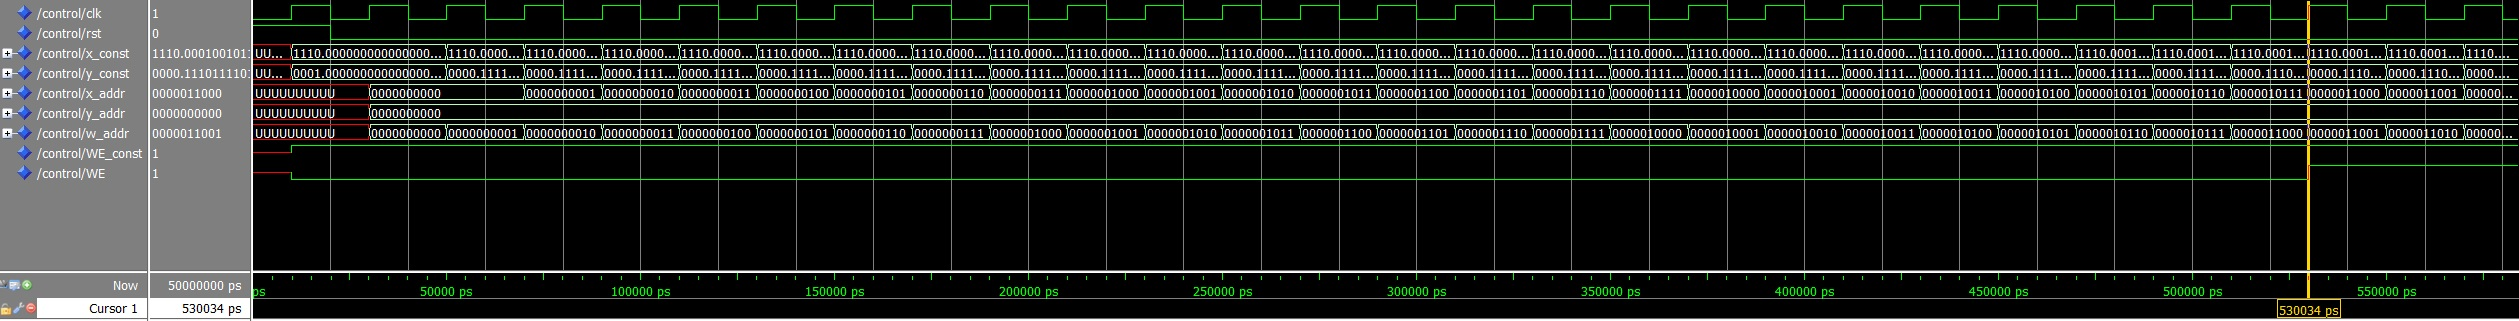
\includegraphics[width=6in]{Control}
\caption{Simulation of the first clock cycles of the control logic.}
\end{figure}
\subsubsection{Math}
The math unit was simulated early in the design process when the exact number of stages possible was not known. It is for this reason that 23 rather than 24 stages appear in the simulation results. The iteration output was as expected.
\begin{figure}[H]
\centering
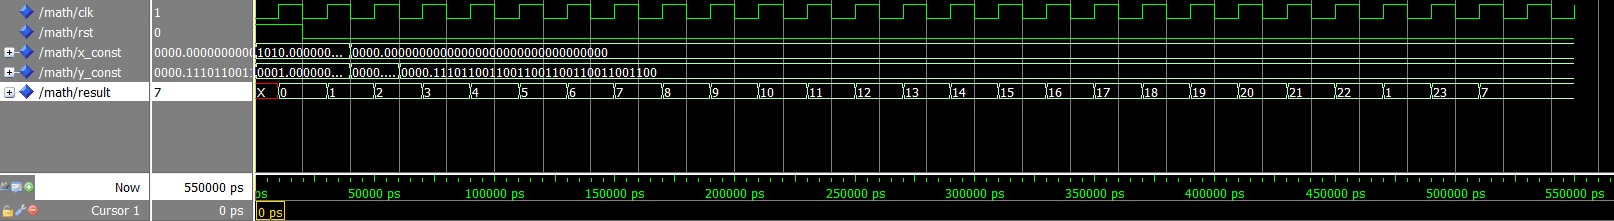
\includegraphics[width=6in]{Math}
\caption{Waveform for 23 stage pipeline.}
\end{figure}
\subsection{Hardware}
The project easily fits onto a Cyclone IV device and synthesis runs with just a few warnings. The reset function is required to load the correct constant values into RAM for the first image. Some issues with the control logic were debugged using the hardware. One issue still remains with the project when running on hardware. Table 4 lists the user inputs on the DE2-115 board.
\begin{table}[H]
\centering
\framebox[6in]{\begin{tabular}{r | l }
$Input$ & $Function$ \\ \hline
KEY0&Global reset when pressed.\\
KEY1&Zoom when pressed and released.\\
KEY2&Vertical zoom: Press and hold while KEY1 is pressed to zoom on upper part of screen.\\
KEY3&Horizontal zoom: Press and hold while KEY1 is pressed to zoom on right side of screen.\\
\end{tabular}}
\caption{User inputs.}
\end{table}
\subsubsection{Synthesis}
The synthesis of the project revealed that the stages of the math unit were taking up twice the 9 bit multipliers expected. Since all values used are 36 bit fixed point, it was assumed 4 multipliers would be used per multiplication and 12 per stage. This turned out to be exactly half the actual value of 24 9 bit multipliers per stage. Synthesis was rerun on the Mandelbrot component individually, but the result was the same. Below is a listing of the synthesis result for the project as a whole.
\begin{figure}[H]
\centering
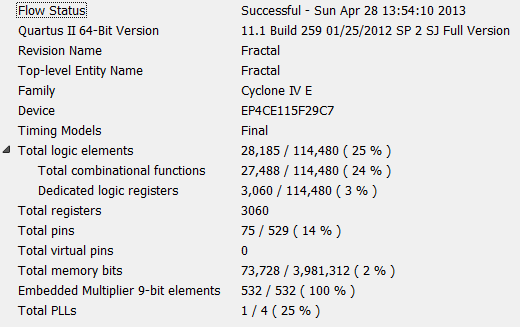
\includegraphics[width=6in]{Stat}
\caption{Synthesis Report.}
\end{figure}
All of the multipliers are used, however 98\% of RAM on the Cyclone IV is still available along with 75\% of the logic units. This means there is plenty of resources for future enhancements. One PLL is used to generate the 65MHz global clock that is required for XGA output.
\subsubsection{Programmed Board}
The project can be loaded onto the DE2-115 board with little issue. One bug remains that does not allow for zooming in on the left side of the screen for the first zoom. The control logic is not easily simulated to the point where user input is considered. The buggy logic is very much like a reverse of the logic used for zooming in on the right side of the screen, thus a quick solution was not found.
\section{Discussion}
\subsection{Successes and Failures}
The VGA output works as expected. No image jittering or distortion is detected. The user interface is consistent and without flaws so long as the zoom x and y buttons are pressed and held before pressing the zoom button. Below is sample output generated just after reset and before zooming.
\begin{figure}[H]
\centering
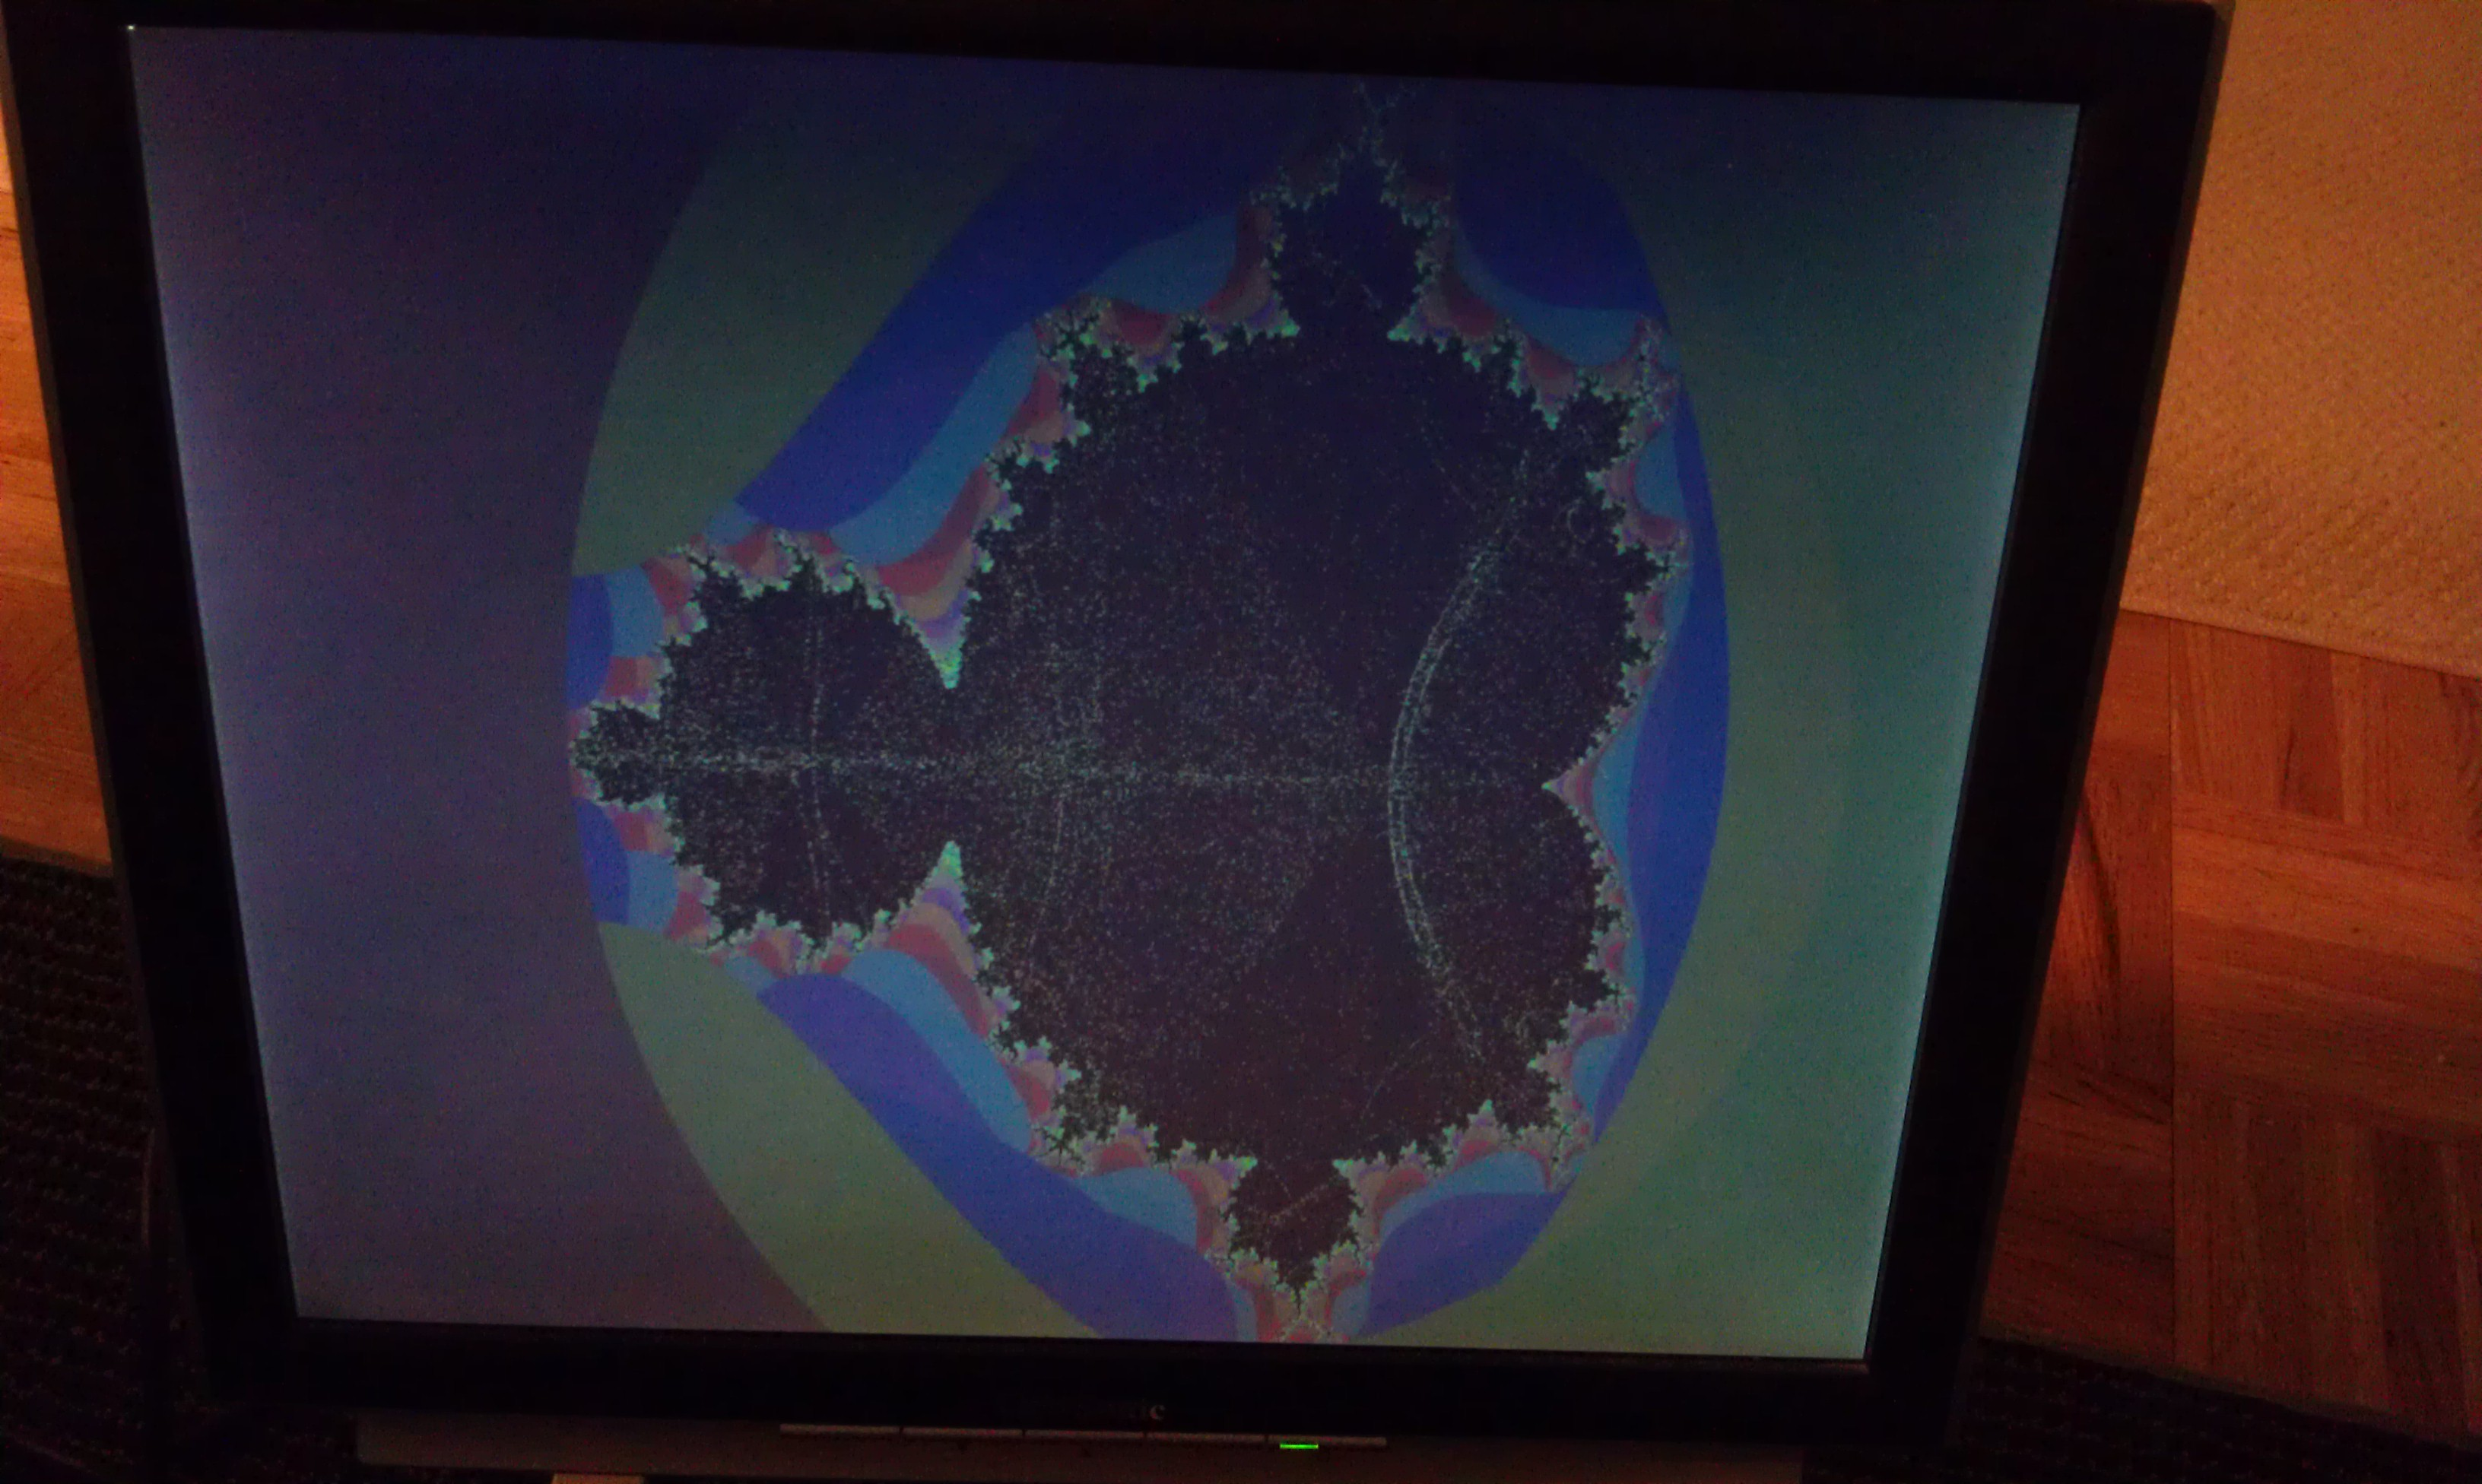
\includegraphics[width=5in]{output}
\caption{Sample output after reset.}
\end{figure}
The only known bug is that zooming in on the left portion of the screen for the first zoom results in a blank screen.
\subsection{Lessons Learned}
A big lesson of this project was to start early, even in the planning stages so that project outcome would be more clear even before writing VHDL. Looking back on the design document, lots of assumptions proved to be wrong while the scope of others was downplayed. A SDRAM controller was just too big of a task, and a parallel architecture not the simplest route to success. The project was easily completed by one person, and this was due to flexibility in the plans and changing the approach once issues cropped up.

Different approaches could have been utilized when writing the VHDL. Use of more megawizard functions could have reduced the need for some VHDL and the logic units needed to synthesize the design. 

Seeking help early and often from a variety of sources could have solved the problem of too many multipliers being used. There are lots of forums where people with experience converse about design issues and someone may have already encountered this issue. Contacting Altera may have shed some light on the synthesis process and the discrepancy between expected and realized results.
\subsection{Future Improvements}
The project lends itself to improvements that could be made in the future either by upgrading components in the system or improving the existing code.

Changing the FPGA used or using standard logic units for multipliers could lengthen the existing pipeline and thus allow for more iterations per pixel. This would be a very simple change, but one that may produce a better image. The way in which the output is generated, as seen in the memory controller listing in section 2.3.3, could be changed to produce a red color only image that may look sharper. Changing the FPGA used might also allow for clocking the datapath faster, if the new FPGA allows for clock selection. The memory controller would then be clocked faster for writes, and then slower when reading out for VGA output. This would reduce flicker where a black screen can sometimes be seen. The Cyclone IV used in this project simply did not have the capability to support multiple global clocks.

A paralleled architecture is an improvement that could be made to the code and run on the same hardware. Using the same Mandelbrot component, one could add multiplexing and demultiplexing components to the datapath. The number of iterations could be increased since the memory architecture already assumes 16 bit values. This improvement may add delay to the calculations required for generating each image, but the resulting image would be much more detailed.

More user interaction could be possible by using other parts of the DE2-115 board. Zooming with mouse or keyboard input to the PS2 or USB ports could allow for zooming in on particular points in the complex plane rather than one of four quadrants. This change would only affect the control logic and more specifically the F and G states.

\section{Conclusion}
Generating fractals and in particular the Mandelbrot Set is possible on the Cyclone IV E FPGA. Fixed point math may be used with the addition of external libraries. User interaction is intuitive when using just four pushbuttons. The project was completed by one person over the course of two months, but more work upfront in researching the design would have led to less discrepancy between the planned and resulting design. 

\section{References}
http://vhdl.org/fphdl/ Support for fixed point arithmetic in pre-VHDL 2008 tools such as Quartus II.

http://stackoverflow.com/questions/9701456/multidimensional-array-of-signals-in-vhdl Arrays of elements (used in Math unit).

http://codelead.se/who-needs-vram-anyway Similar Verilog project.

http://rosettacode.org/wiki/Mandelbrot\_set Examples in computer programming languages.
\end{document}
